\begin{savequote}[75mm]
Do not lose your faith -- for a mighty fortress is our mathematics. It shall rise to the occasion. It always has. 
\qauthor{Stanislaw Ulam (1909-1984)}
\end{savequote}

\chapter{Selecting Suitable Sites}
\label{chapter 1}

\newpage
 
\section{Selecting Suitable Sites for Artificial Groundwater Recharge Basins}

\newthought{The first principle challenge} which must be overcome in an attempt to quantify the life-cycle energy water usage efficiency of a proposed new water reuse system involving artificial groundwater recharge is the need to develop of a systematic method for selecting sites that are suitable for the construction of the requisite recharge basins. This problem of \textit{selecting suitable sites}, relative to one or more criteria of suitability, is one which is extremely common within the domain of Geographic Information Science (GIScience). And indeed, the need to develop consistent methodologies and capable tools for achieving this purpose were among the core research goals which initially stimulated the early development of the field \cite{Tomlin1979,Tomlin1994,Malczewski1999}.
 
\section{Multi-Criteria Site Suitability Analyses}

One methodology which has emerged as a reliable means of approaching this type problem, and the one which was adopted for the purposes of this dissertation, is a procedure known as multi-criteria site suitability (MCSS) analysis. MCSS analyses mathematically combine two or more input geographic data layers that each correspond to some independent measure of site suitability for a given landuse application \cite{Bolstad2005}. The output of this MCSS computation is a single geographic data layer in which the value at each location represents a composite measure of overall site suitability relative to all of the independent criteria, simultaneously \cite{Hopkins1977, Collins2001}.  

MCSS analyses are typically conducted using geographic information that has been stored in a continuous raster format. This means that prior to conducting this type of analysis each of the input geographic data layers that are to be used must be preprocessed relative to some reference raster format so as to ensure the feasibility and consistency of the MCSS computation. For example, in order for the computation to be feasible: all of the input data layers must have the same number of cells and occupy that same geographic extent. Similarly, in order for the computation to be consistent: the ordinality and the scaling of the values in each raster must accurately reflect the relative weighting and directionality of each independent suitability criterium.
 
Geographic information system (GIS) software packages are commonly used to conduct both these types of data preprocessing operations as well as the MCSS computation itself \cite{Malczewski2004, Malczewski2006}. This is because they provide pre-built functions which facilitate the import of spatial data layers from disparate sources as well as the manipulation of geographic data layers such that they satisfy the previously mentioned feasibility and consistency constraints. Often, the MCSS analyses itself is not the endpoint goal of a given research effort however. Many times, MCSS analyses are used as inputs to some other, more complex, numerical optimization model \cite{Church2002}. This situation is frequently encountered in the fields of operations research (OR) and location science (LS) where MCSS outputs are used to derive network topologies or linear programming constraints for optimization problems related to vehicle routing, flow maximization, or facility location \cite{Huber1985, Church1992}. 

\section{The MCSS Data Preprocessing Workflow}
    
The generic data preprocessing workflow for MCSS analysis involves one or more of the three phases illustrated conceptually in ~Figure \ref{fig:Preprocessing}. First, all of the input spatial data layers must be checked to determine whether or not they possess the same coordinate system. If they do not, a single reference coordinate system must be chosen by the analyst to function as the standard for all of the input layers. The choice of this reference coordinate system is generally driven by the scale of spatial domain involved as well as the desired tradeoff between distance versus areal measurement error. The output of this \textit{Reproject} operation is a set of duplicate  data layers that are all projected as the reference coordinate system. 

The second phase of the workflow involves clipping the various input data layers on the basis of their overlap with some reference spatial extent. This reference extent may correspond to the boundaries of a single input layer or may be arbitrarily designated by the analyst. The output of this \textit{Clip} operation is a set of duplicate data layers that all have the same spatial extent as the reference extent. 

The third and final phase of the workflow involves rasterizing all of the input layers such that they have the same cell size and cell alignment. During this phase, input data layers that are stored using a different geographic data model must be algorithmically converted into a raster based representation. As part of this algorithmic conversion process, a reference cell size, usually corresponding to the largest cell size contained within the input data layers, is used as a reference. The output of this \textit{Rasterize} operation is a set of duplicate layers that all share the same cell size and cell alignment as the designated reference.
    
        \begin{figure}[!h]
            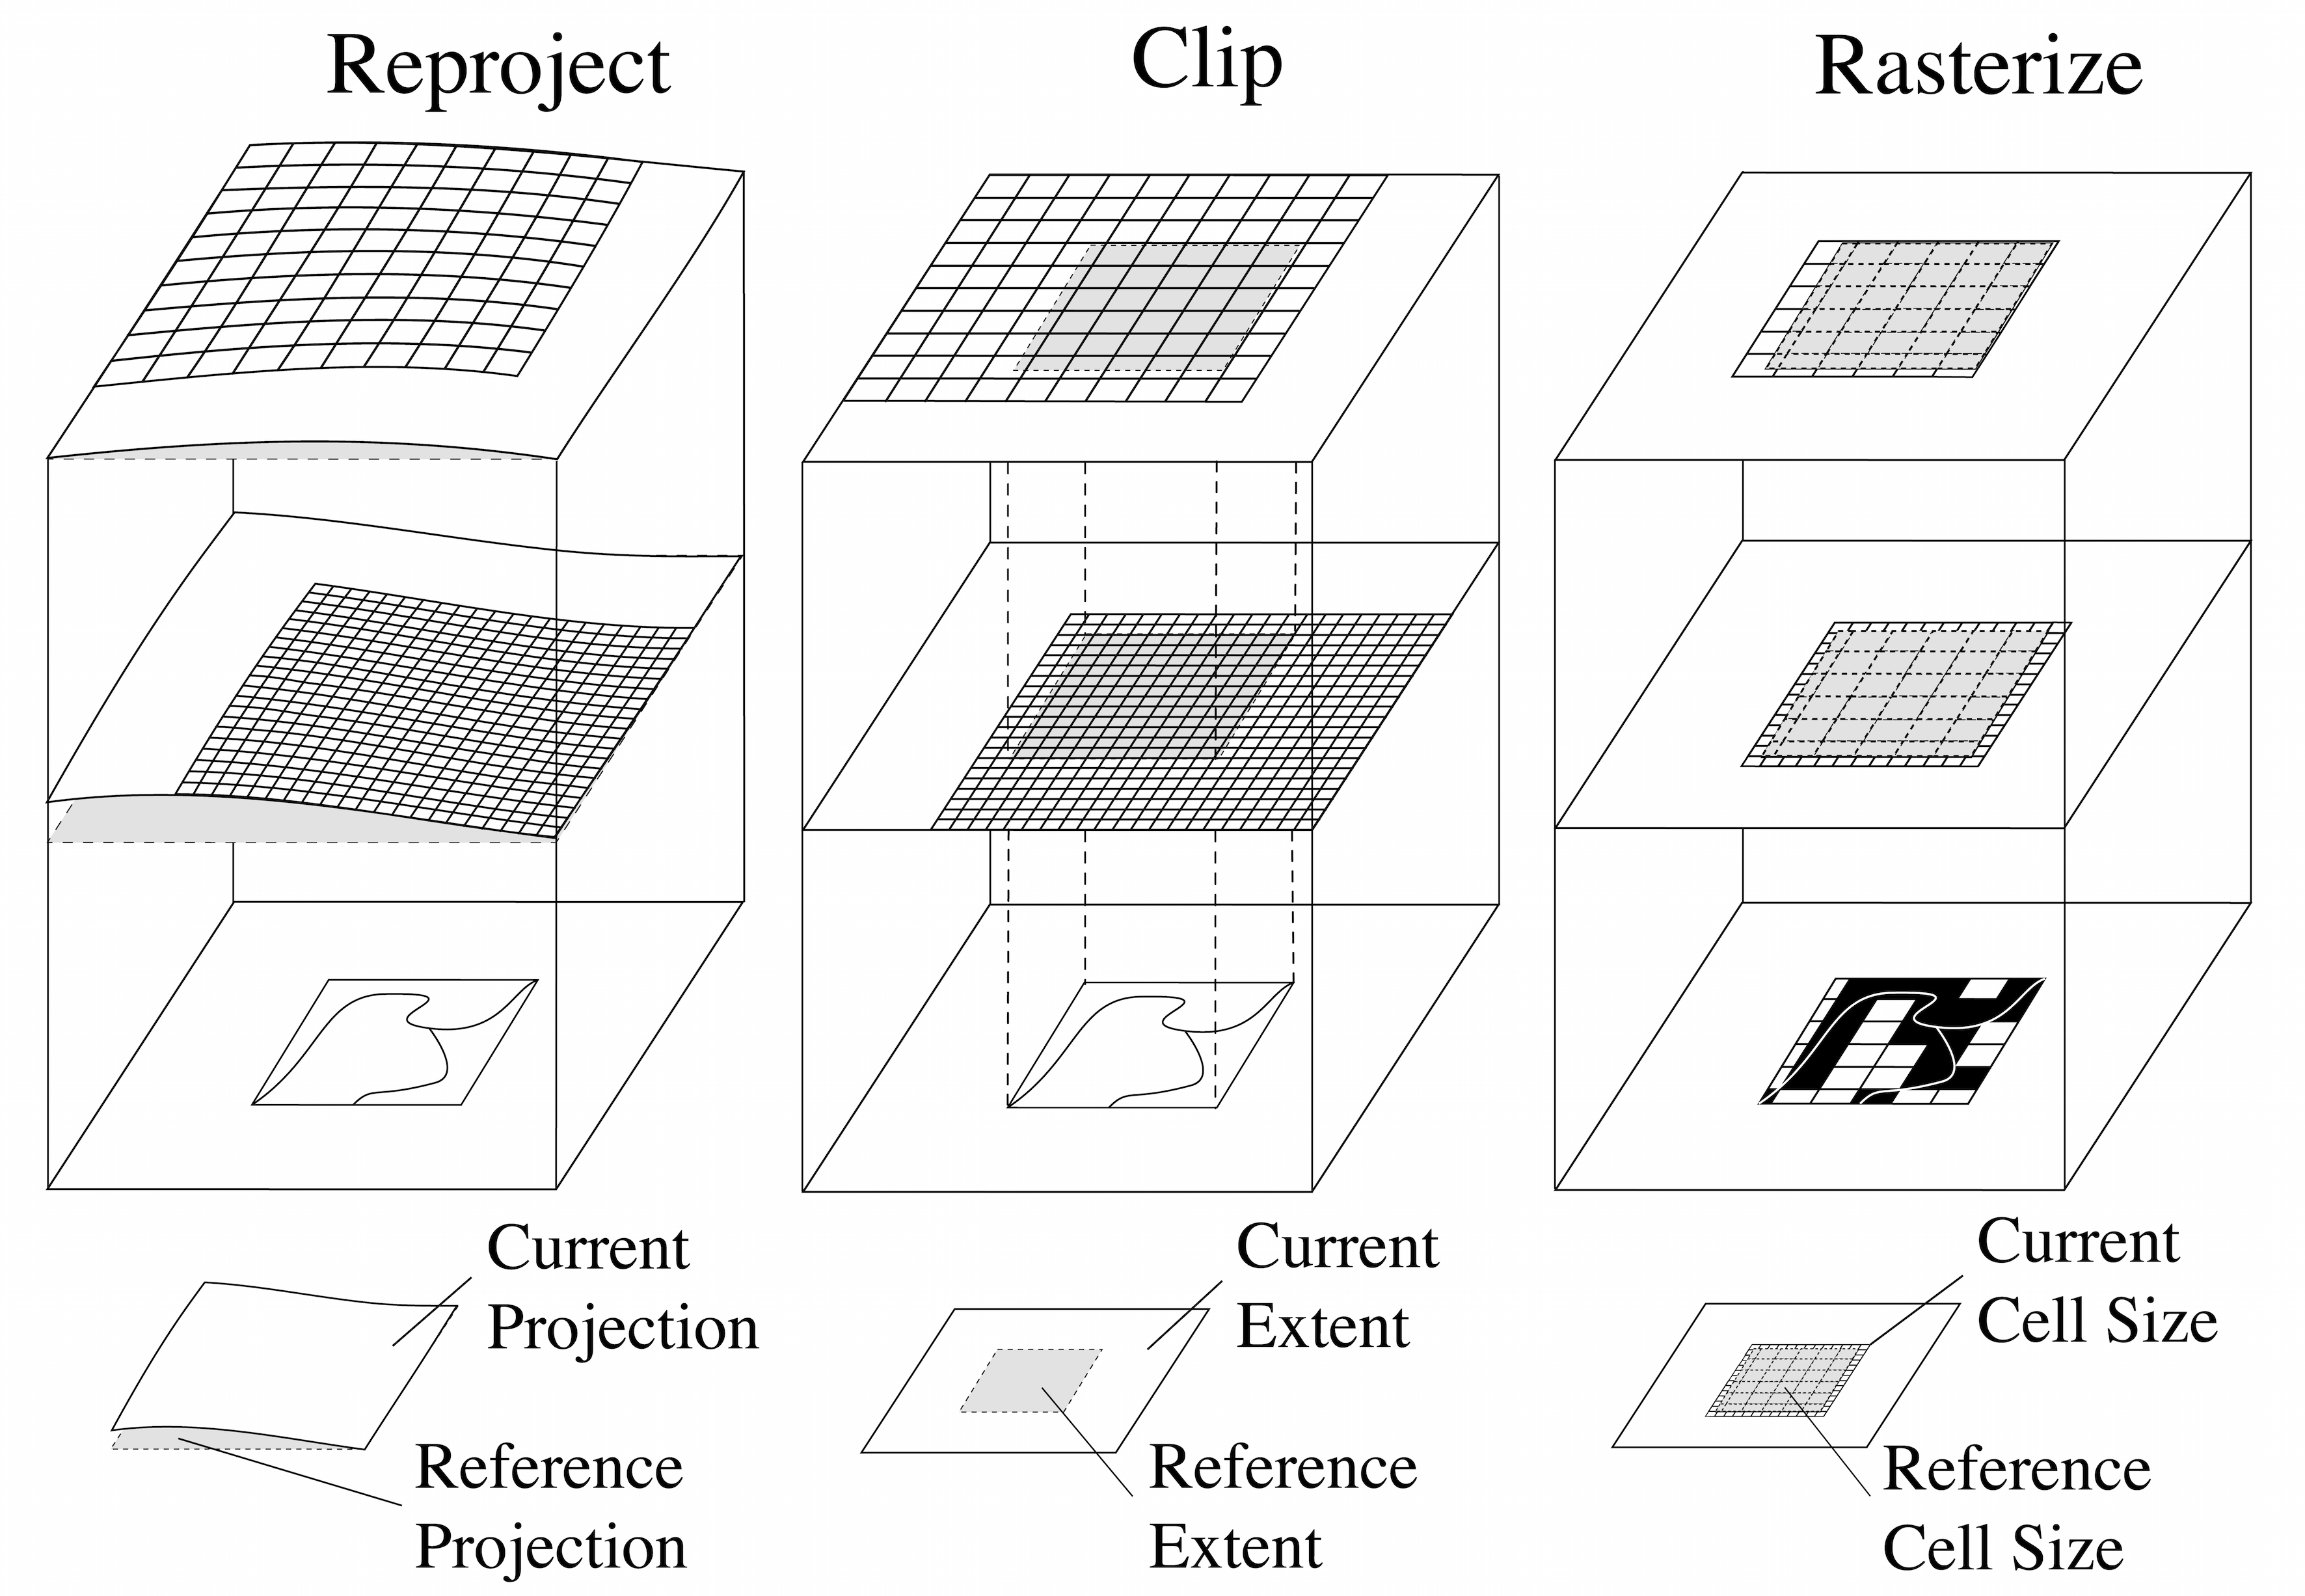
\includegraphics[width=5.5in]{figures/data_processing_workflow.png}
             \caption{Conceptual illustration of the input data preprocessing operations and workflow phases typical to most MCSS analyses}
              \label{fig:Preprocessing}
        \end{figure} 
        
\section{The MCSS Computational Workflow}
    
Instead of executing the MCSS data preprocessing steps manually for each of the five case study regions that were going to be investigated as part of this dissertation, the decision was made to implement a more generic data preprocessing software framework which enable any researcher -- not necessarily the author of this dissertation --  to conduct a similar analysis for any region in which sufficient input data was available. These tools, which shall be described in subsequent sections, were implemented in the the MATLAB$^{\circledR}$ programming environment and have been made publicly available as a source code repository hosted at: \url{https://github.com/ericdfournier/WOSS}. The control flow logic which guided their development is described in the pseudocode in ~Figure \ref{fig:Pseudocode}.

Prior to the initiation of any MCSS analysis the researcher must provide a set of raw spatial data input files and designate a set of spatial reference criteria. Once these requirements are met, all of the input spatial data files are then subjected to a sequence of conditional statements. Depending upon the result of these conditional statement evaluations various transformation functions are then sequentially applied to the input data files so as to produce a set of outputs whose projection, spatial extent, cell size, and cell alignment all match a set of designated spatial reference criteria.

        \begin{figure}[!h]
        \begin{centering}
        \label{euclid}
            \begin{algorithmic}[1]
                \Procedure{Preprocess Input Data}{}
            
                    \ForAll{$input$}
                        \If{$input_{prj} \neq reference_{prj}$}
                            \State $input = Reproject(input)$
                        \ElsIf{$input_{ext} \neq reference_{ext}$}
                            \State $input = Clip(input)$
                        \ElsIf{$ isRaster(input_{type}) \neq True$}
                            \State $input = Rasterize(input)$
                        \ElsIf{$input_{cs} \neq reference_{cs}$}
                            \State $input = Resize(input)$
                        \EndIf
                        \State $output = input$
                    \EndFor
                    \State \textbf{return} $output$
                    
                \EndProcedure
            \end{algorithmic}
        \end{centering}
        \caption{Control logic for MCSS input data preprocessing workflow.}
        \label{fig:Pseudocode}
        \end{figure}
            
The current version of the toolset only supports the reprojection of input spatial data layers that are represented using geographic coordinates -- i.e. data stored in latitude \& longitude coordinate space. This constraint not only limits the directionality of the reprojection operation but also greatly simplifies the spatial interpolation routines required for the rasterization process. The authors plan to lift this restriction in future versions of the toolset as the MATLAB$^{\circledR}$ language's native support for forward map projection as well as the automated parsing of standard formatted spatial reference data strings improves.   
            
Following the preprocessing of the spatial data inputs, the next phase of the MCSS modeling process is the user guided reclassification of the data values in each layer into a quantitative measure of suitability for the land use application in question. Routines are provided in the toolset to facilitate this process. Among these are an automated histogram equalization based reclassification procedure which assigns suitability values ensuring an even distribution of all the values contained within some range across all of the areas within the spatial data layer. Other tools allow the user to manually specify the range of the bins used for the reclassification of raw input data values to site suitability rankings. 

\section{The Software Toolset Repository Architecture}
    
The directory structure of the WOSS toolset repository is illustrated in ~Figure \ref{fig:Directory}. Below the top level root directory are four standalone files: (1) a \textit{\textbf{LICENSE.md}} file, (2) a  \textit{\textbf{README.md}} file, (3) a \textit{\textbf{GUI.m}} file and (4) \textit{\textbf{GUI.fig}} file. The first two files contain the software license and general repository usage guidance, respectively. The third and fourth, are the source code files supporting the standalone graphical user interface that visually guides a user through this same data preprocessing workflow.

        \begin{figure}[!h]
            \dirtree{%
             .1 $\dots$/.
             .2 LICENSE.md.
             .2 README.md.
             .2 GUI.m.
             .2 GUI.fig.
             .2 src/.
             .3 *.m (functions).
             .2 smp/.
             .3 data/.
             .4 vector/.
             .5 *(filename)/.
             .6 *.shp, *.shx, *.dbf, *.prj.
             .4 raster/.
             .5 *(filename)/.
             .6 *.tif, *.tfw.
             .2 output/.
             .3 binary/.
             .4 *.mat.
             .3 raster/.
             .4 *.tif, *.tfw.
            }
            \caption{Directory tree structure for the toolset repository. Filetypes required for input data and automatically generated as output data are shown.}
              \label{fig:Directory}
        \end{figure}
        
Also below the top level root directory are the following three subdirectories: (1) \textit{\textbf{src/}}, (2) \textit{\textbf{smp/}}, (3) \textit{\textbf{output/}}. The \textit{\textbf{src/}} directory contains the MATLAB$^{\circledR}$ source code m-files comprising the toolset's various functions. The \textit{\textbf{smp/}} directory contains MATLAB$^{\circledR}$ .m-file scripts that can optionally be called to automate the execution of multiple data preprocessing workflows. The \textit{\textbf{/smp/data/}} directory contains two sub-directories: \textit{\textbf{vector/}} and \textit{\textbf{raster/}}. Each of these houses the corresponding sub-directories, one for each vector and raster based raw input spatial data files provided by the user. The tiles used for each of these \textit{\textbf{*(filename)}} sub-directories are automatically assigned to the outputs generated by the tool. The supported vector input filetype is the ESRI shapefile format. Alternatively, the supported raster input file type is the open source GeoTiff format. Finally, the \textit{\textbf{output/}} directory contains two sub-directories: \textit{\textbf{binary/}} and \textit{\textbf{raster/}}. These subdirectories comprise the default destination locations for all of the outputs generated by the toolset tools. Outputs can be produced in either the mat-file MATLAB$^{\circledR}$ ASCII-binary format or in the same GeoTiff format as the input raster data.

The toolset supports the use of composite raster data sets which are made up of multiple, possibly overlapping, individual raster data tiles. It does this by performing a bounding box intersection test for each input raster data tile with the reference spatial domain. For those tiles whose bounding boxes are found to intersect that of the reference domain, values are iteratively compiled into a new composite mosaic data layer made up of, potentially several, individual tiles. This makes it possible to use input raster data layers that are of arbitrarily high resolution covering large geographic domains.

\section{An Example Implementation}
    
The raw input datasets which were selected for the example implementation were collected from several publicly available sources. A brief topical description of each source as well as a link to its source web repository is given in ~Figure \ref{fig:DataSources}. In addition to these raw input data sources, a number of derived data products are generated automatically from the digital elevation model (DEM) for use in this particular case study analysis. These derived products include: slope \& aspect.

    \begin{figure}[!h]
        \begin{center}
            \begin{tabular*}{0.45\textwidth}{l | l | l}
                \textbf{Type} & \textbf{Category} & \textbf{Source} \\ \hline
                Vector & Resource Areas & \href{http://www.atlas.ca.gov/download.html}{Cal-Atlas} \\ \hline
                Vector & County Boundaries & \href{http://www.atlas.ca.gov/download.html}{Cal-Atlas} \\ \hline
                Vector & Surface Geology & \href{http://www.atlas.ca.gov/download.html}{Cal-Atlas} \\ \hline
                Vector & Road Network & \href{http://www.atlas.ca.gov/download.html}{Cal-Atlas} \\ \hline
                Vector & STATSGO Soils & \href{http://water.usgs.gov/GIS/metadata/usgswrd/XML/ussoils.xml#stdorder}{USGS} \\ \hline
                Vector & State Park Boundaries & \href{http://www.atlas.ca.gov/download.html}{Cal-Atlas} \\ \hline
                Vector & Stream Reaches & \href{http://viewer.nationalmap.gov/viewer/}{National Map} \\ \hline
                Vector & Street Network & \href{http://www.atlas.ca.gov/download.html}{Cal-Atlas} \\ \hline
                Vector & Surface Water Storage & \href{http://www.atlas.ca.gov/download.html}{Cal-Atlas} \\ \hline
                Raster & Crop Data Layer & \href{http://www.nass.usda.gov/research/Cropland/SARS1a.htm}{USDA} \\ \hline
                Raster & Digital Elevation Model & \href{http://viewer.nationalmap.gov/viewer/}{National Map} \\ \hline
                Raster & NLCD Landcover & \href{http://viewer.nationalmap.gov/viewer/}{National Map} \\ 
           \end{tabular*}
    \end{center}
    \caption{Table of input data sources used in the case study MCSS model for artificial groundwater recharge applications.}
    \label{fig:DataSources}
    \end{figure}

\section{The Geographic Unit of Analysis}
    
The geographic unit of analysis selected for this example implementation is the US Geologic Survey (USGS) Hydrologic Unit Code (HUC) level five watershed. Specifically, the level five watershed areas contained within the administrative boundaries of the state of California. According to the USGS:

    \blockquote{\textit{The United States is divided and sub-divided into successively smaller hydrologic units which are classified into four levels: regions, sub-regions, accounting units, and cataloging units. The hydrologic units are arranged or nested within each other, from the largest geographic area (regions) to the smallest geographic area (cataloging units). Each hydrologic unit is identified by a unique HUC consisting of two to twelve digits based on the levels of classification in the hydrologic unit system. \cite{Seaber1987}}}
    
The level five designation within this HUC framework is comprised of closed contiguous regions possessing an average area of $588$ square kilometers. These level five HUC designated areas are often referred to as the HUC-10 watersheds because of their use of a ten digit unique numerical identification code. Within the state of California, there are 1,040 individual HUC-10 watersheds. These watersheds are non-overlapping and have been derived algorithmically from the national elevation dataset by USGS scientists according to the method described by \cite{Seaber1987}.
    
\section{Graphical User Interface}
   
The WOSS toolset can be interactively parameterized via the the GUI depicted in Figure \ref{fig:GUIpart1}. The GUI is presented as a three step workflow, with each step building iteratively upon the product of the previous one to generate a final composite output. The first step involves the user providing the directory location of the shapefile from which the reference geometry will be selected. The user is presented with the option of specifying an alternative \textit{\textbf{Overlay Shapefile}} that can be used to aid in the selection of this reference area. The second step involves the use of this overlay shapefile to generate an interactive map window that will appear to the user once it is time for the reference boundary to be selected. It should be noted that the reference shapefile always provides the source data from which the actual selection is made. 

Next, the user is then prompted to input parameter values for two fields. The first corresponds to the grid density that will be used to generate all of the output layers. The default setting for this parameter is $1,169.99$. This grid cell density roughly corresponds to cells that are ($100$ $m$ x $100$ $m$) or $10,000$ $m^2$  within the latitude range bounding the state of California. The second input parameter value corresponds to the attribute field name in the reference shapefile that will be used for the output reference grid encoding. The attribute field must be of numerical type. 

         \begin{figure}[!h]
            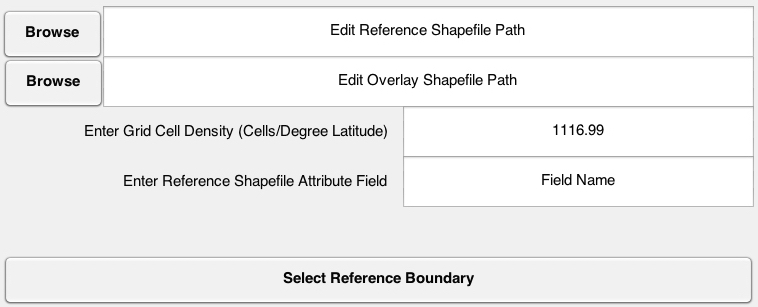
\includegraphics[width=5.5in]{figures/gui_fig1.jpg}
            \caption{An overview of Step \#1 in the GUI based workflow: parameterizing the reference grid.}
            \label{fig:GUIpart1}
        \end{figure}

Once the user correctly provides all of these inputs they are then allowed to move onto the second step of the workflow which by clicking on the \textit{\textbf{Select Reference Boundary}} button. During this step a map axis is generated in which the geometry information for the overlay shapefile is drawn on screen as shown in Figure \ref{fig:GUIpart2}. The user may then select their desired reference polygon by simply clicking on the appropriate location within the map. The latitude longitude coordinates corresponding to this selection are automatically used to extract the containing polygon from the reference shapefile. This polygon is then automatically converted to a reference grid with the cell density and attribute field encoding parameters designated by the user.

         \begin{figure}[!h]
            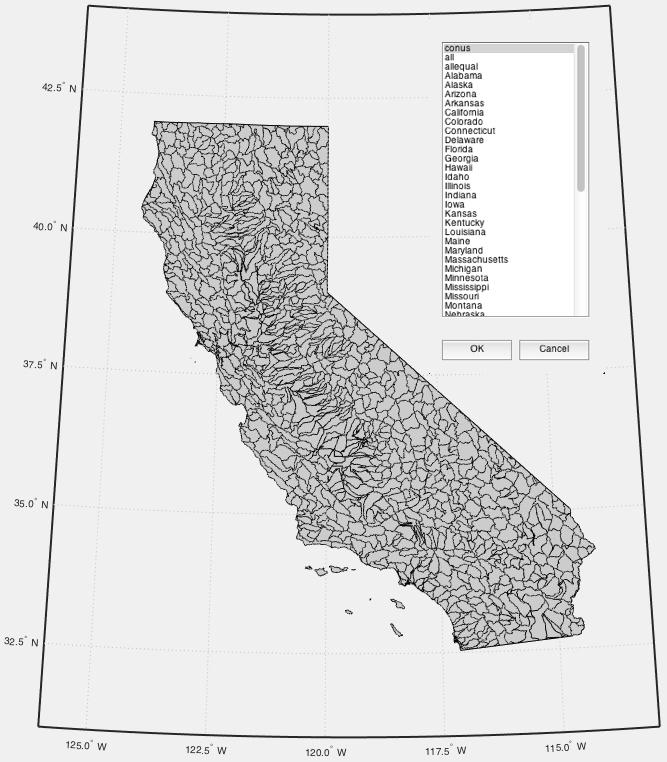
\includegraphics[width=5.5in]{figures/gui_fig2.jpg}
            \caption{An overview of Step \#2 in the GUI based workflow: selecting the reference polygon from the overlay shapefile geometry.}
            \label{fig:GUIpart2}
         \end{figure}

The third step of the GUI based workflow, shown in Figure \ref{fig:GUIpart3}, involves the user providing the directory locations of the various spatial data inputs that are to be processed. These inputs should be organized according to the general directory layout described in the preceding section. Once these top level directory locations have been provided, the names of the raw input data layers are automatically populated into the accompanying tables and the users are prompted to provide one more parameter value for each vector and raster data category. For the raw input raster datasets, the users are requested to input to the table the numerical encoding of any \textit{NaN} values. If none is present the field may simply be left blank. For the raw input vector datasets, the users are requested to input the text encoded name of the attribute fields on the basis of which the output grid layers will be encoded. Here again, as with the generation of the reference grid, these attribute field names should correspond to numerically encoded values.

         \begin{figure}[!h]
            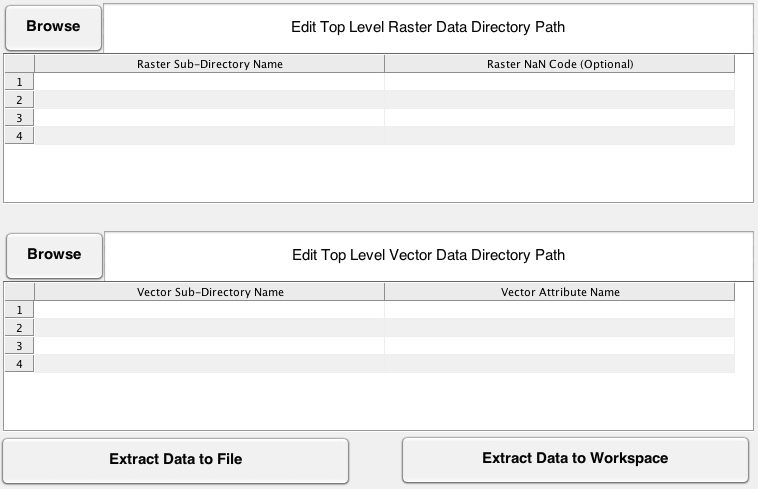
\includegraphics[width=5.5in]{figures/gui_fig3.jpg}
            \caption{An overview of Step \#3 in the GUI based workflow: selecting the reference polygon from the overlay shapefile geometry.}
            \label{fig:GUIpart3}
         \end{figure}
         
Following successful completion of the various data processing steps the user is then allowed to choose whether they want to save the output layer stack directly into the MATLAB workspace via the \textit{\textbf{Extract Data to Workspace}} button, or to disk in a file encoded as either as a set of GeoTiff (.tiff) formatted rasters or a single MATLAB binary (.mat) via the \textit{\textbf{Extract Data to File}} button.
    
\section{The WOSS Model Outputs}
    
Figure \ref{fig:SampleOutput} illustrates a set of sample outputs that were generated by the data preprocessing components of the toolset for an example HUC-10 reference boundary. The reference boundary can either be selected manually, by calling a function which prompts the user to click on map with all of the HUC-10 boundaries drawn on it, or automatically, by specifying the 10-digit code corresponding to the desired HUC-10 watershed. The toolset processes generate an output layer stack -- the individual component layers of which are illustrated in the colored inset map panels. Only layers for which there is at least one non-empty data value are included in the generated outputs. Thus, the number of output components may vary depending upon the coverage of the input data layers relative to the domain of the reference boundary. For vector data inputs, the values which are contained in the output are those corresponding to a single attribute field selected by the user. This field must be either a real or coded numeric data type as the raster data format does not support the native representation of categorical variables.
    
        \begin{figure}[!h]
            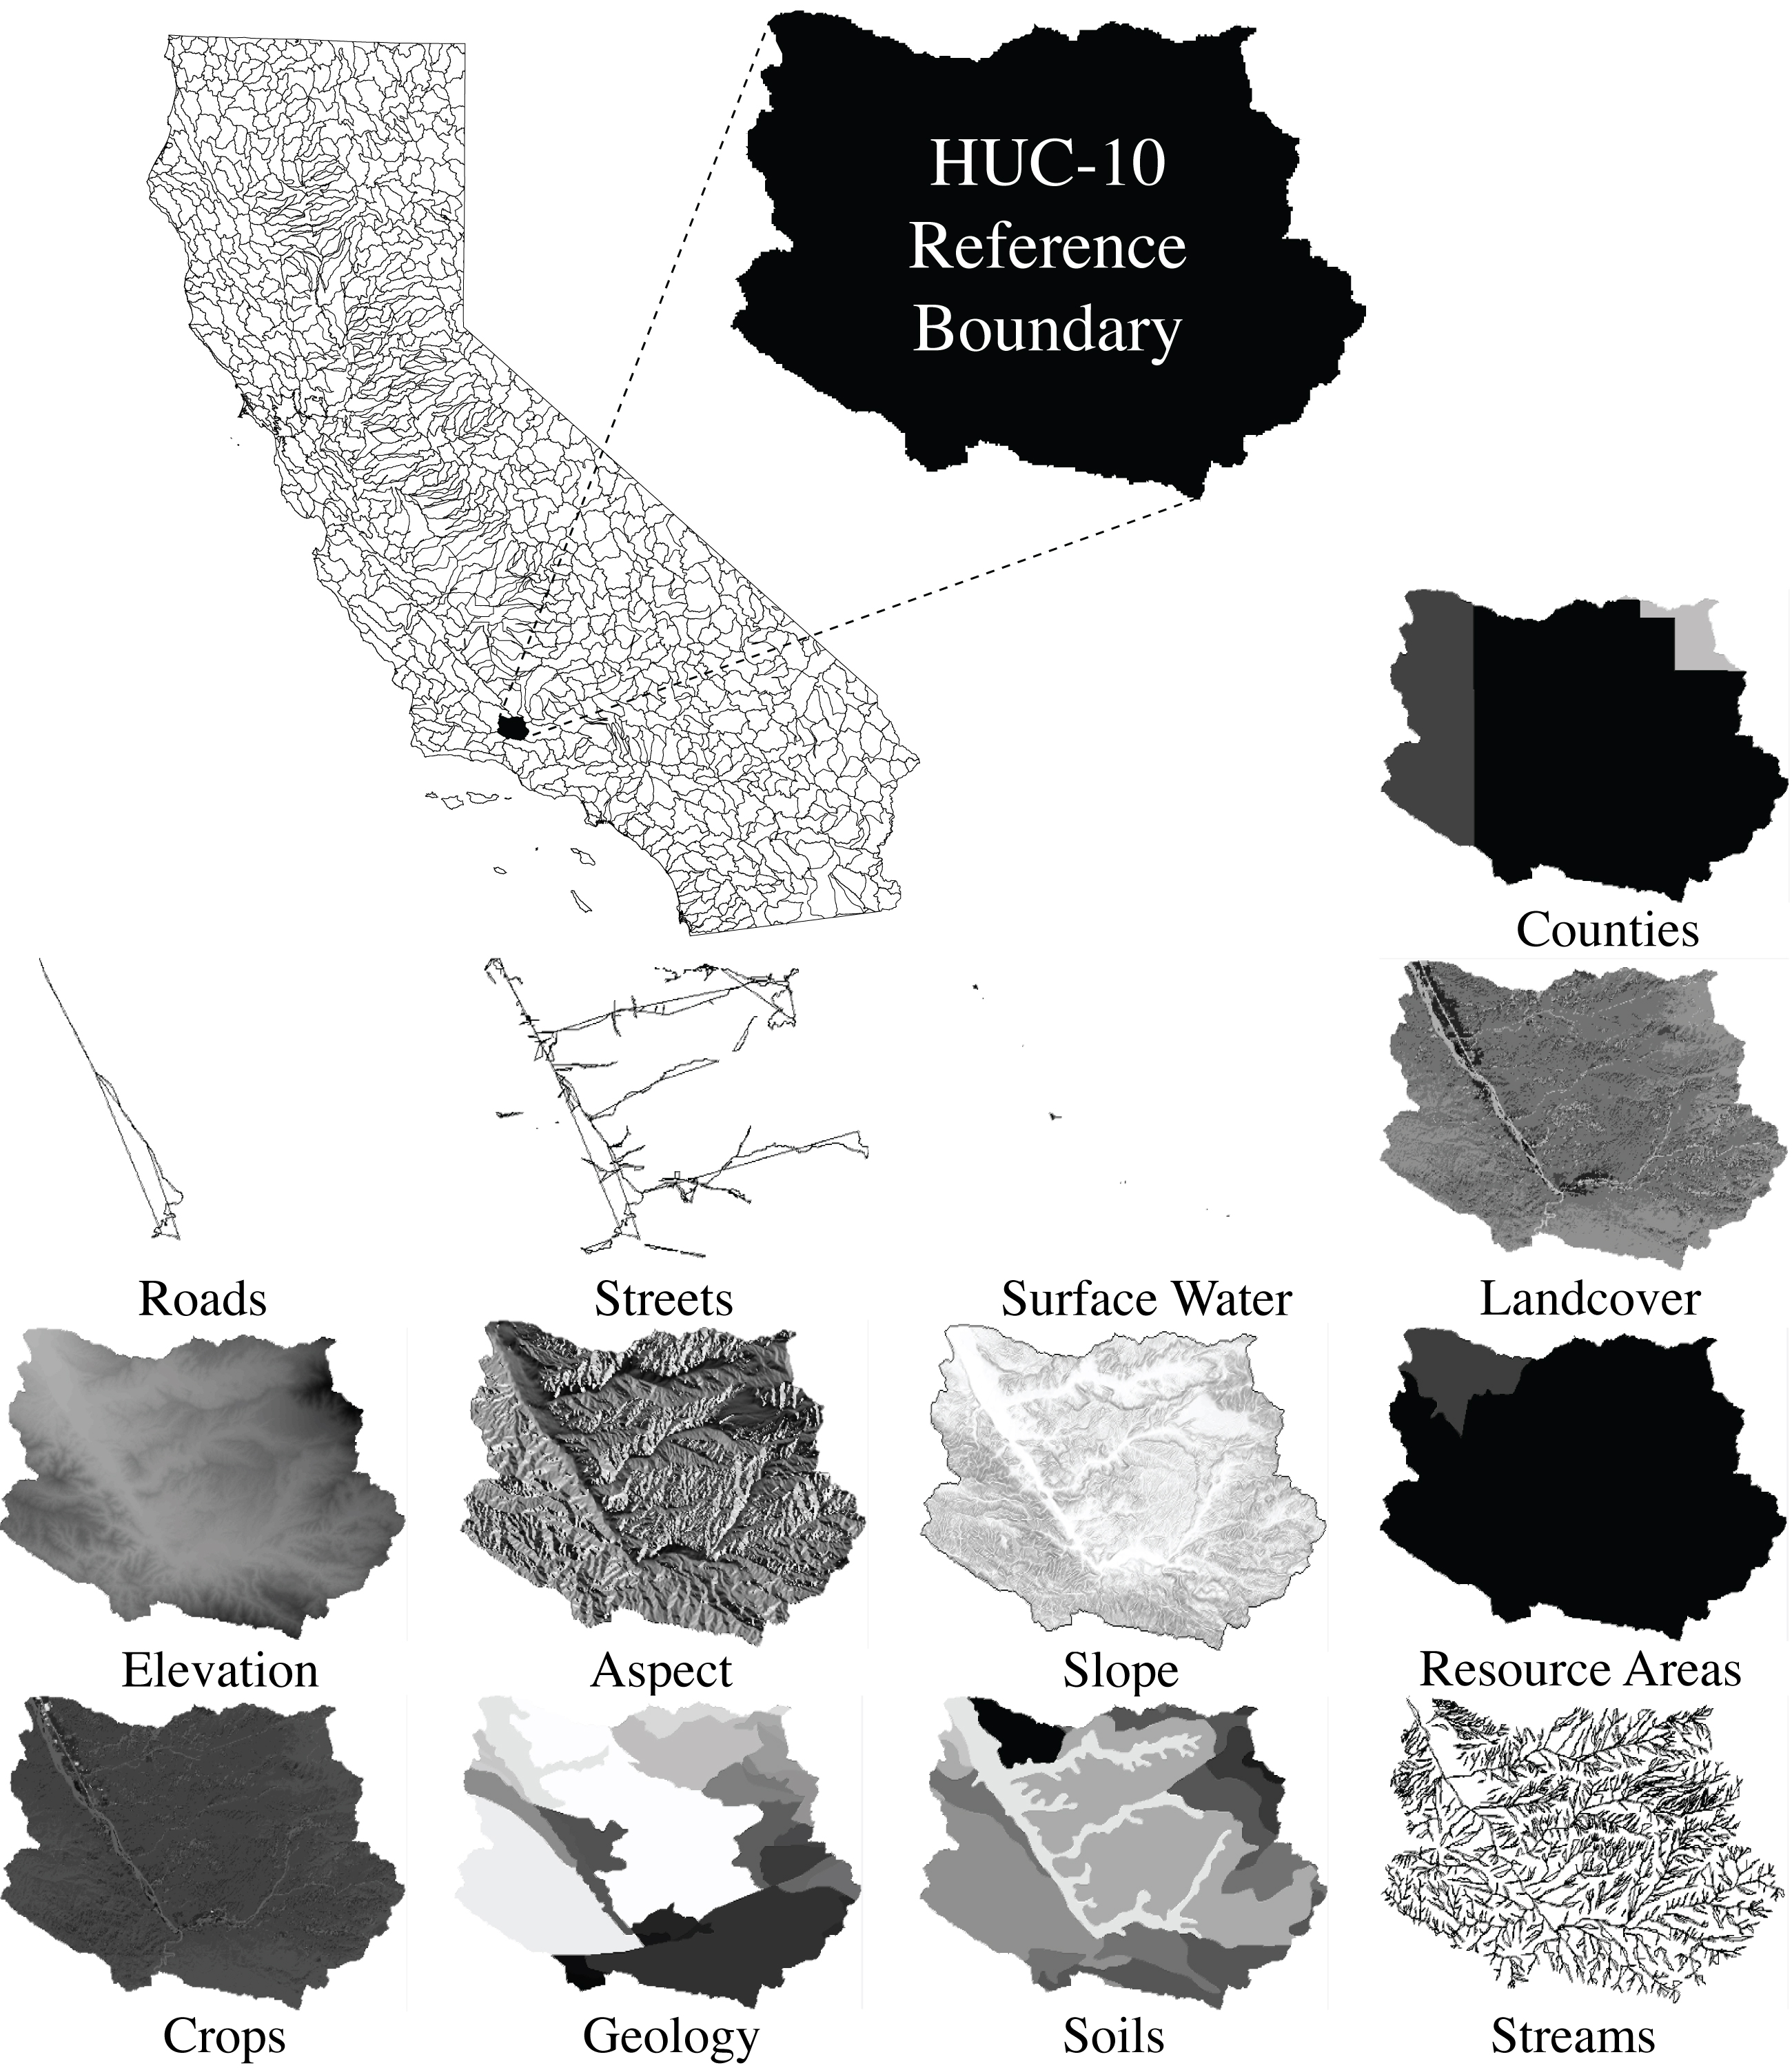
\includegraphics[width=5.5in]{figures/example_data_output.png}
            \caption{Graphical Illustration of the WOSS Model Outputs for Reference HUC-10 Boundary}
            \label{fig:SampleOutput}
        \end{figure}

The toolset structure allows for the automated repetition of this data preprocessing workflow for a large number of reference boundaries. In this case study implementation, for example, the toolset was used to prepare a single such output layers stack for each of the 1,040 individual HUC-10 reference boundaries contained within the state of California. With these outputs, a corresponding the MCSS analysis could then be easily conducted for any or every such HUC-10 watershed in the State.
    
\clearpage   